\title{MECH 45X\\Dossier 11 - Code}
\author{Team 26}

\documentclass[12pt,letterpaper,titlepage]{article}
\usepackage[letterpaper, portrait, margin=1in]{geometry}
\usepackage[final]{pdfpages}

\begin{document}
\maketitle
% ****
% _all
% ****
The code for running for running the sensor package is:
\begin{verbatim}
'_all.ino'.
\end{verbatim}
This code runs all of the sensors, prints data to Serial connection, and publishes the data to ThingSpeak. The code is presented on the following pages. The logic to the code is as follows:
\begin{enumerate}
\setlength{\itemsep}{1pt}
\item Turn on the sensor package
\item Turn on CO2 sensor
\item Read from MRT, SHT, and VOC sensors while CO2 sensor warms up (PM sensor is off)
\item Read from CO2 sensor
\item Save CO2, MRT, SHT, and VOC average readings
\item Turn off CO2 sensor and turn on PM sensor
\item Read from MRT, SHT, and VOC sensors while PM sensor warms up (CO2 sensor is off)
\item Read from PM sensor and save value
\item Push CO2, PM, MRT, SHT, and VOC readings to ThingSpeak
\item Turn off PM sensor and turn on CO2 sensor
\item Repeat forever
\end{enumerate}
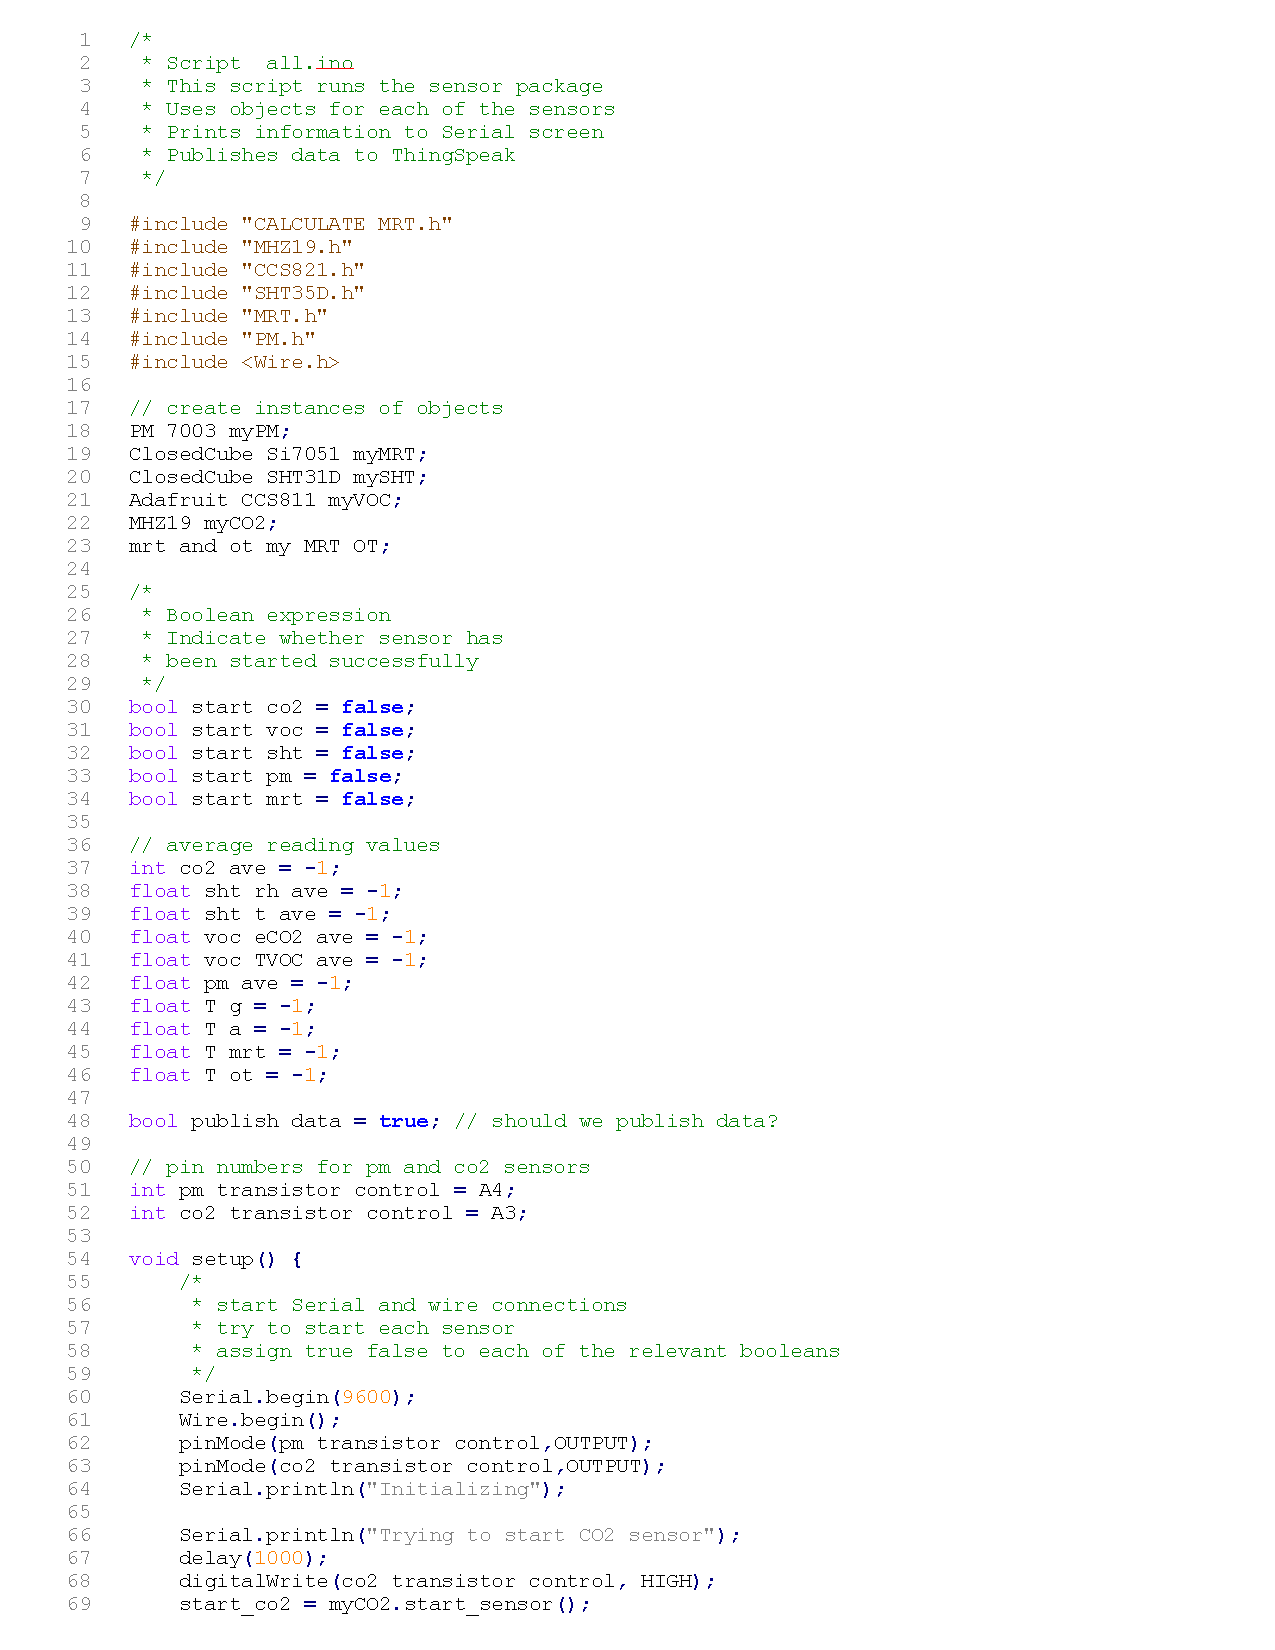
\includepdf[pages=-,pagecommand={},width=\textwidth]{_all.pdf}
% *********************
% _Calculate MRT and OT
% *********************
The code for calculating Mean Radiant Temperature and Operating Temperature is:
\begin{verbatim}
'calculate_MRT.cpp' and 'calculate_MRT.h'
\end{verbatim}
This code uses the globe thermometer temperature, the air temperature, and the convection coefficient to calculate MRT and OT. This code was written entirely by Team 26 using equations from the literature. The .h file is presented first, followed by the .cpp file.
\includepdf[pages=-,pagecommand={},width=\textwidth]{calculate_MRT_h.pdf}
\includepdf[pages=-,pagecommand={},width=\textwidth]{calculate_MRT_cpp.pdf}
% ****
% _PMS
% ****
The code for running the PMS7003 Particulate Matter sensor is:
\begin{verbatim}
'PM.cpp' and 'PM.h'
\end{verbatim}
This code reads from the PM sensor several time and takes an average value of all of the readings. The PMS7003 communicates using a UART connection. This code was written entirely by Team 26. The .h file is presented first, followed by the .cpp file.
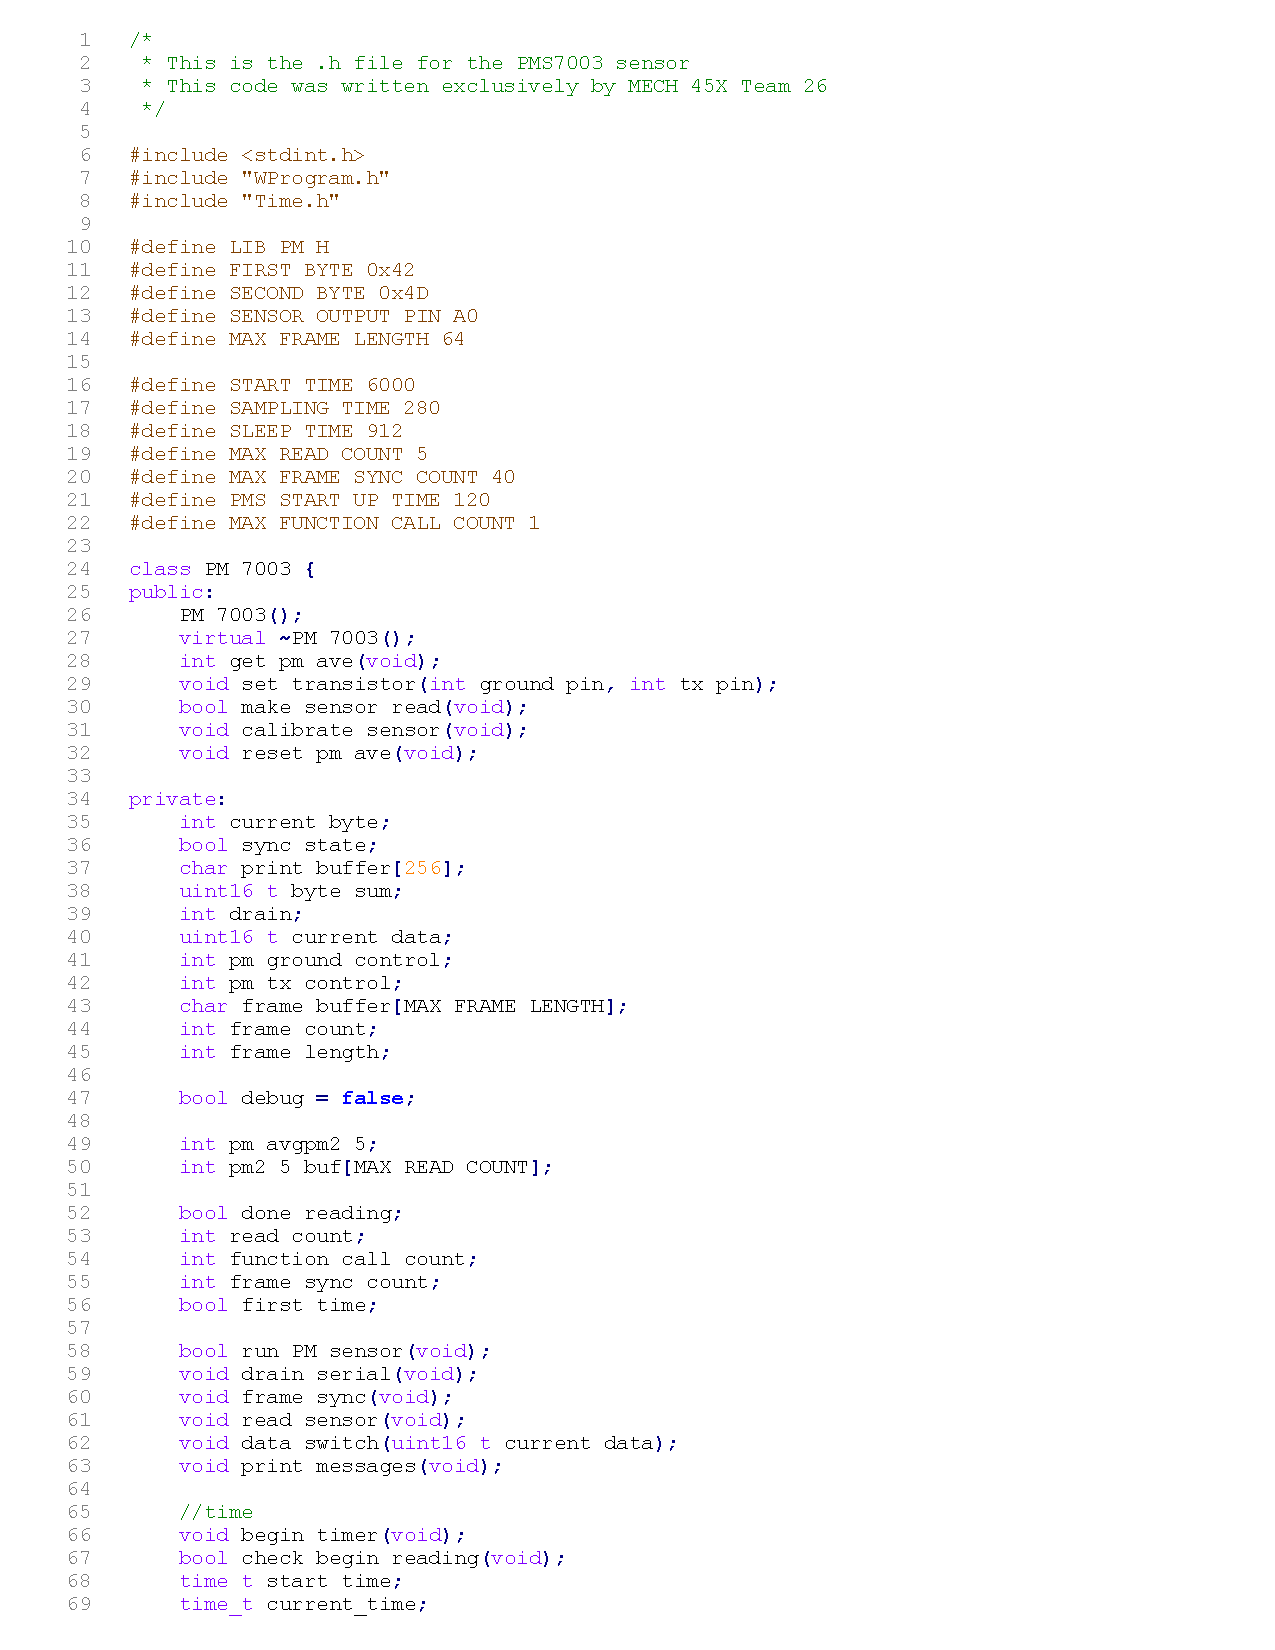
\includepdf[pages=-,pagecommand={},width=\textwidth]{PM_h.pdf}
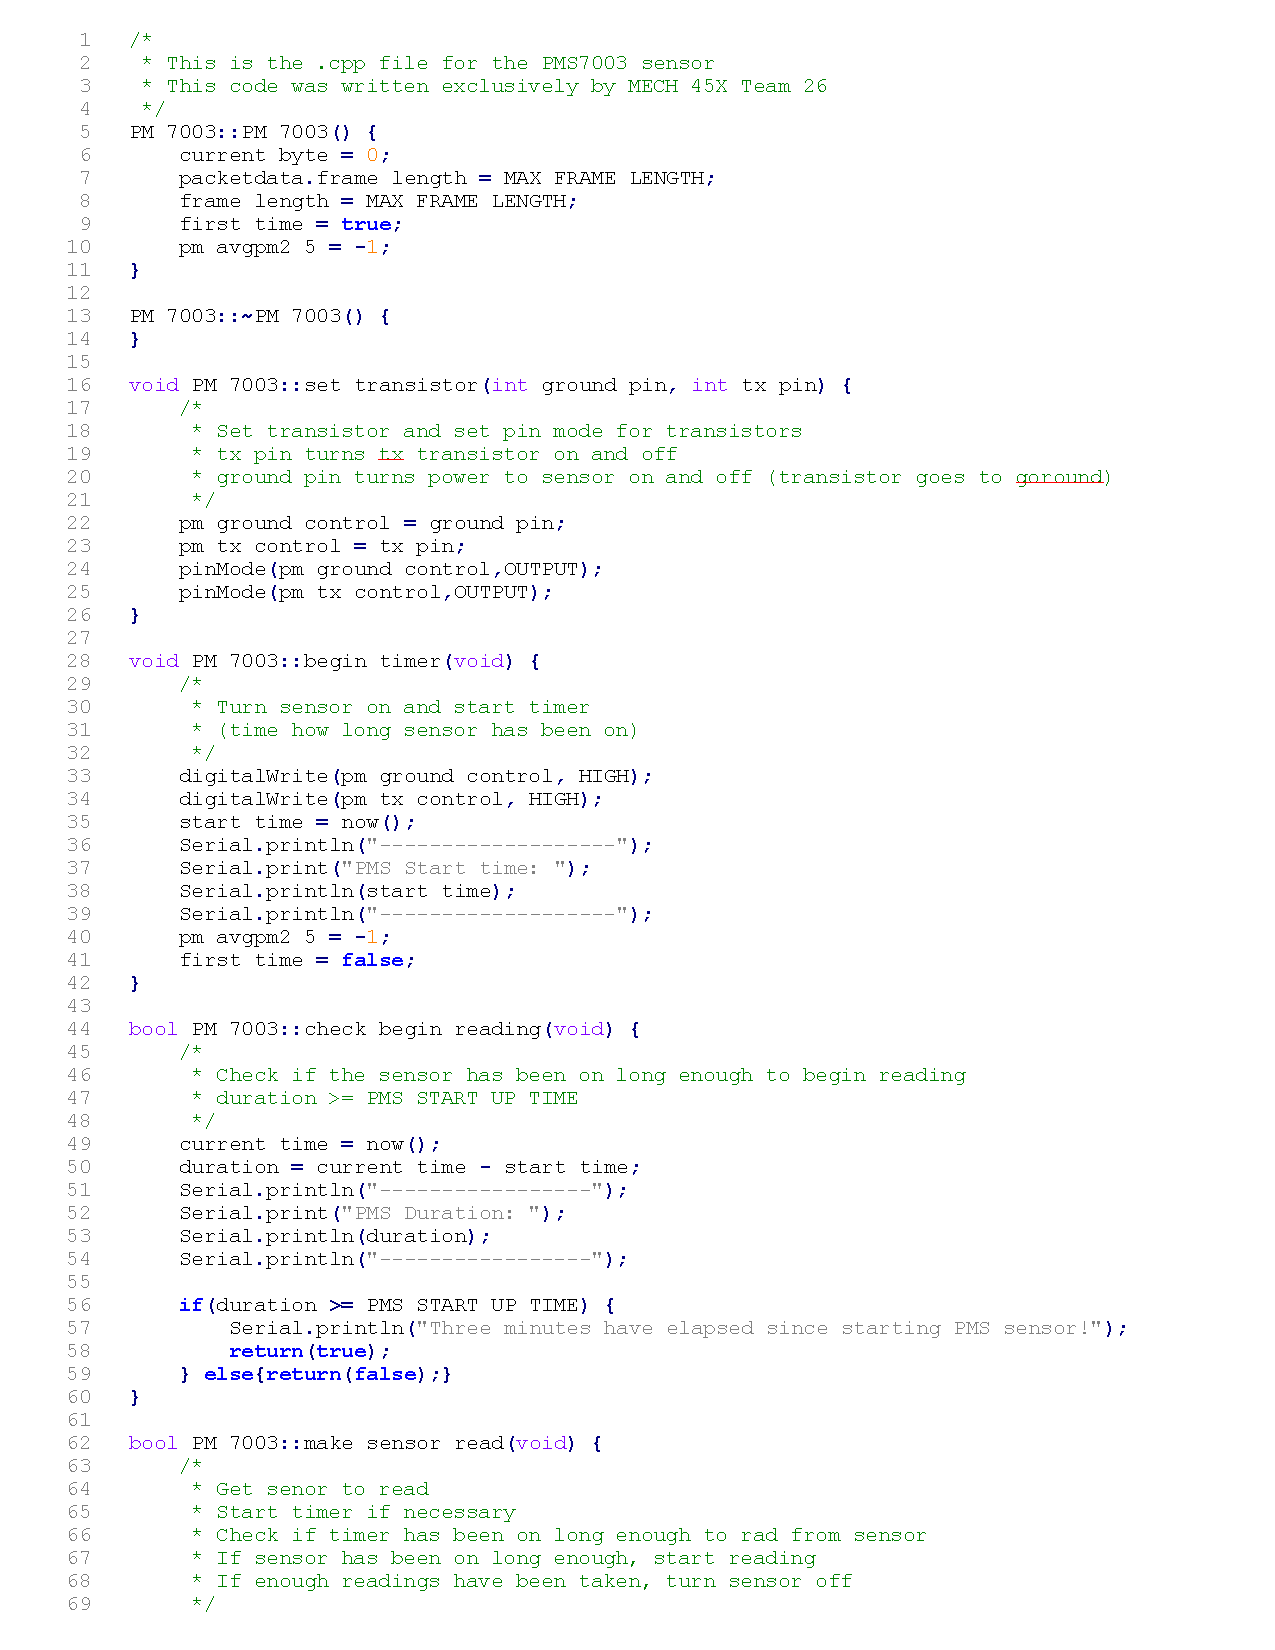
\includepdf[pages=-,pagecommand={},width=\textwidth]{PM_cpp.pdf}
% ****
% _CO2
% ****
The code for running the MH-Z19 CO2 sensor is:
\begin{verbatim}
'MHZ19.cpp' and 'MHZ19.h'
\end{verbatim}
This code reads from the CO2 sensor several time and takes an average value of all of the readings. The MH-Z19 communicates using a UART connection. This code was written entirely by Team 26. The .h file is presented first, followed by the .cpp file.
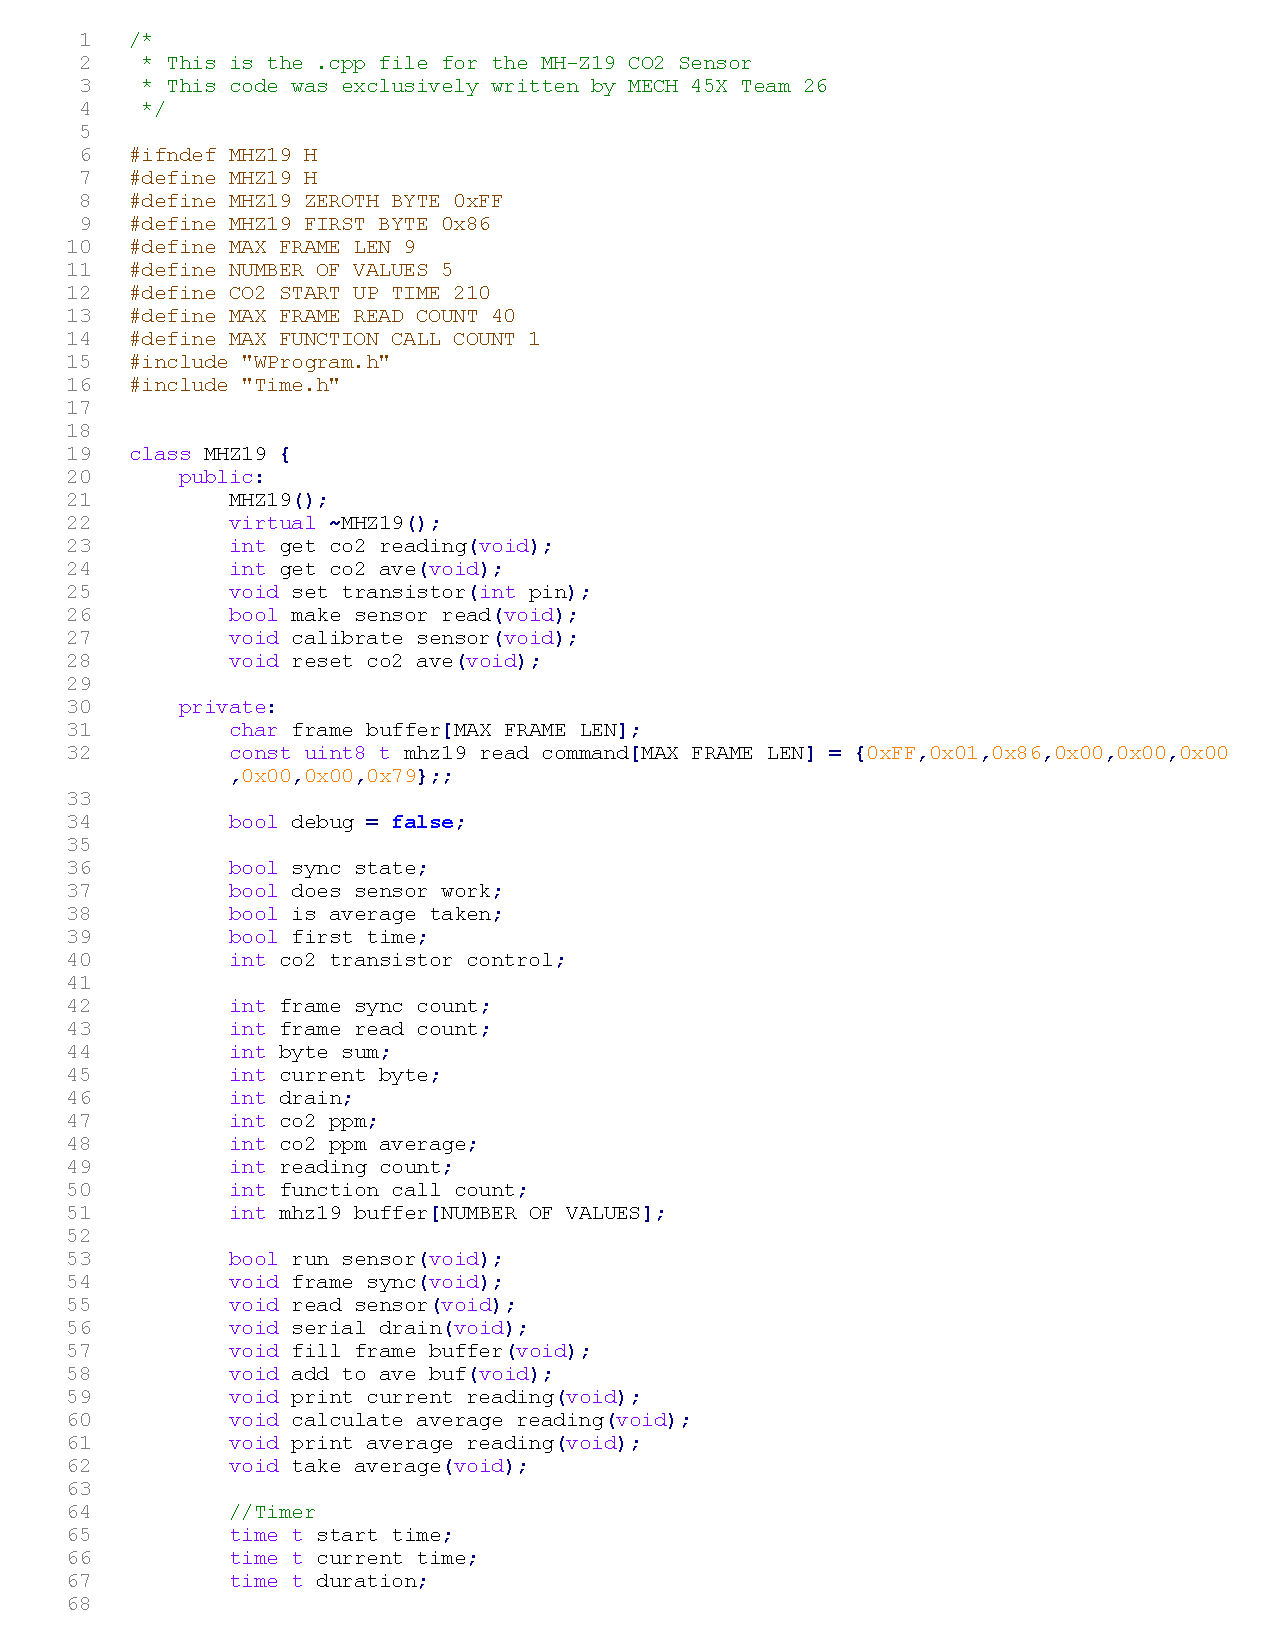
\includepdf[pages=-,pagecommand={},width=\textwidth]{MHZ19_h.pdf}
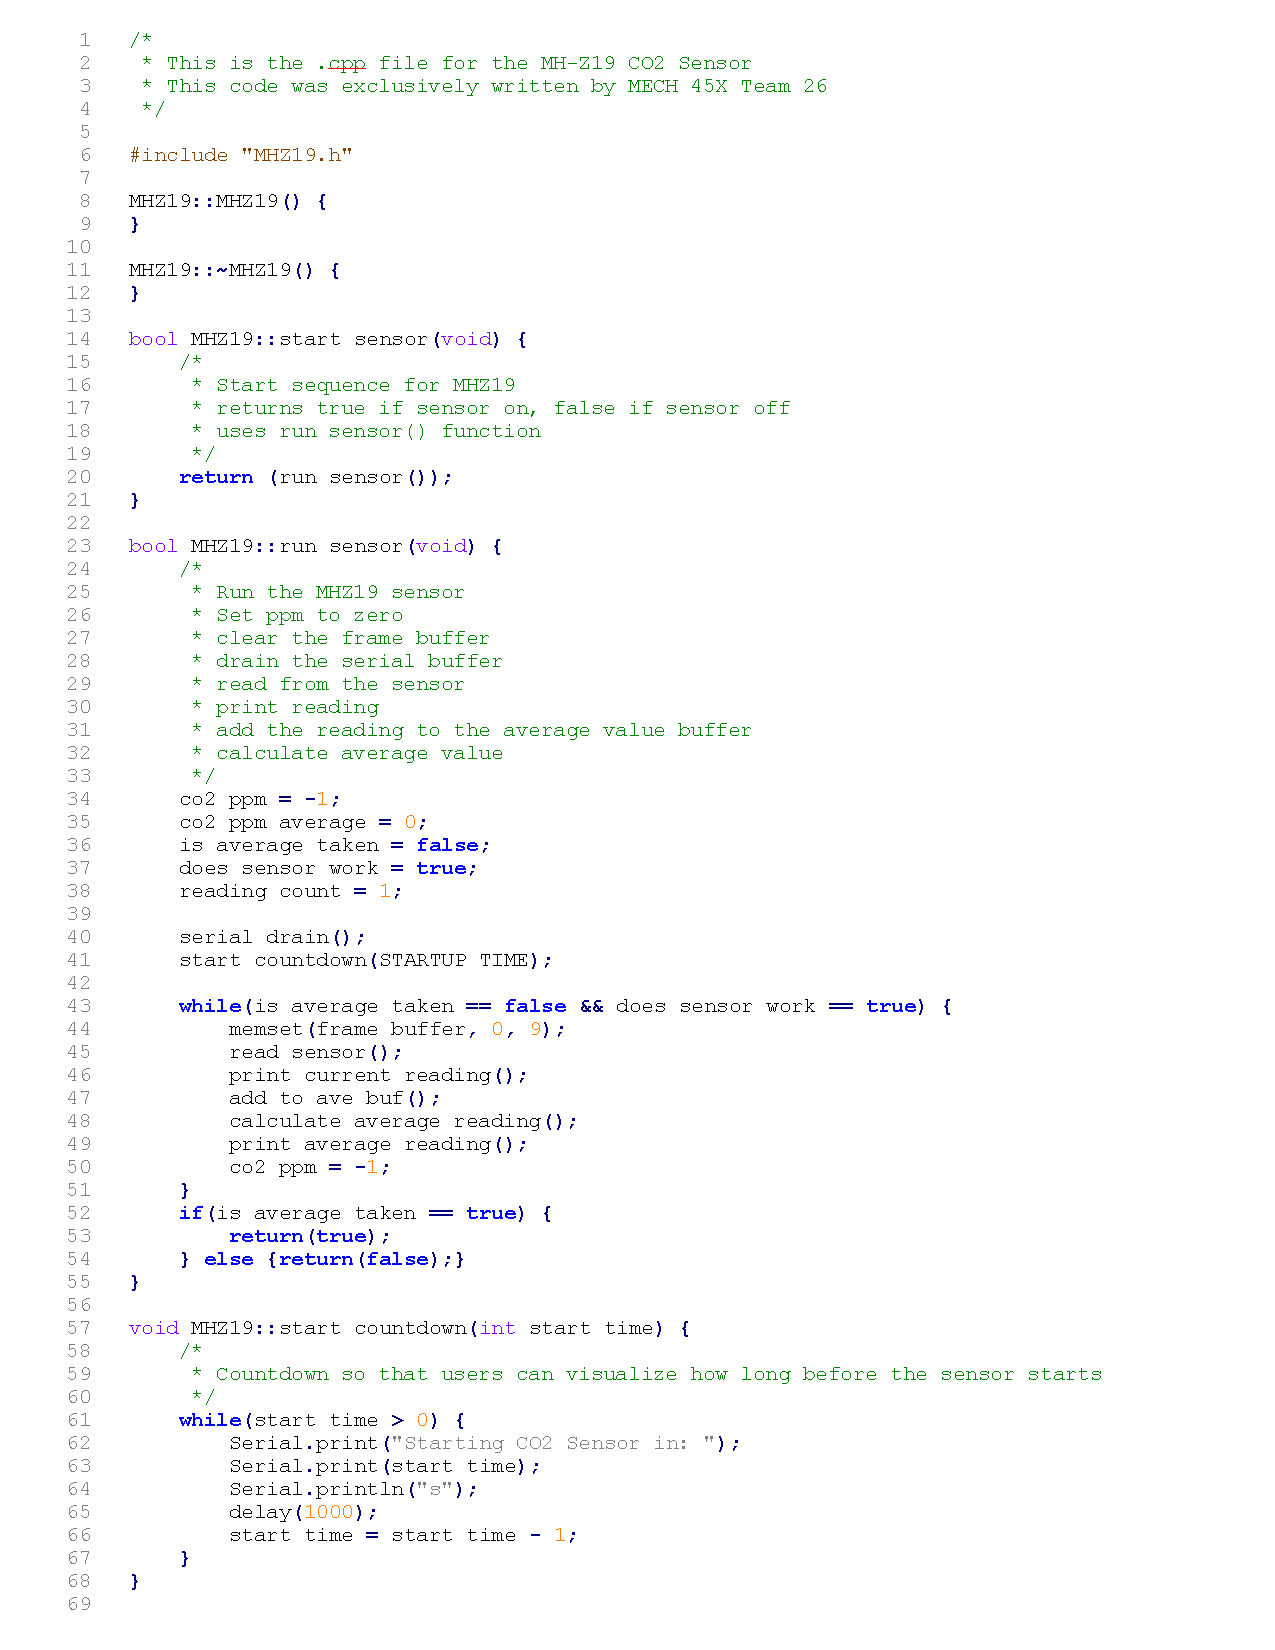
\includepdf[pages=-,pagecommand={},width=\textwidth]{MHZ19_cpp.pdf}
% ****
% _VOC
% ****
The code for running the CCS821 VOC sensor is:
\begin{verbatim}
'ccs821.cpp' and 'ccs821.h'
\end{verbatim}
This code reads from the VOC sensor several time and takes an average value of all of the readings. The CCS821 communicates using an I2C connection. This code was retrieved from:
\begin{verbatim}
https://learn.adafruit.com/adafruit-ccs811-air-quality-sensor
/arduino-wiring-test
\end{verbatim}
The on line library was supplemented by additional methods added by Team 26. The .h file is presented first, followed by the .cpp file.
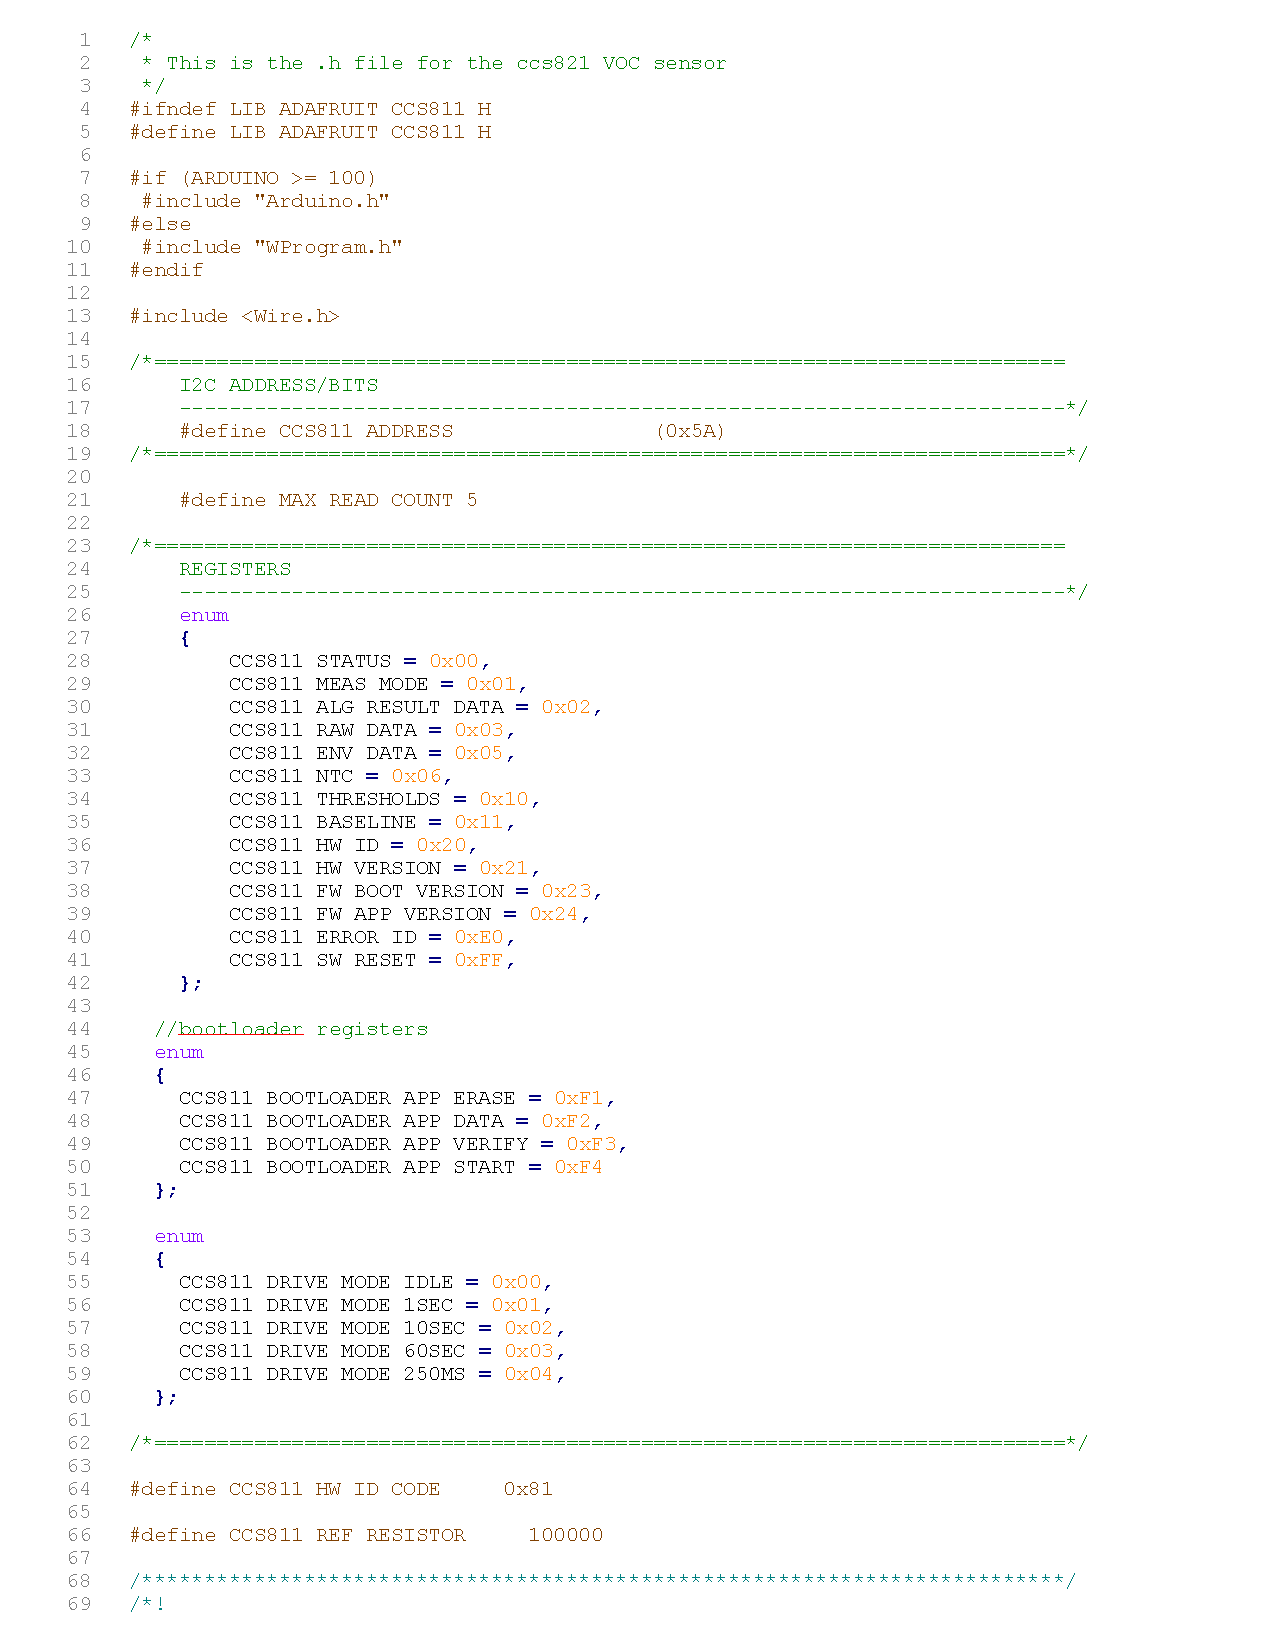
\includepdf[pages=-,pagecommand={},width=\textwidth]{ccs821_h.pdf}
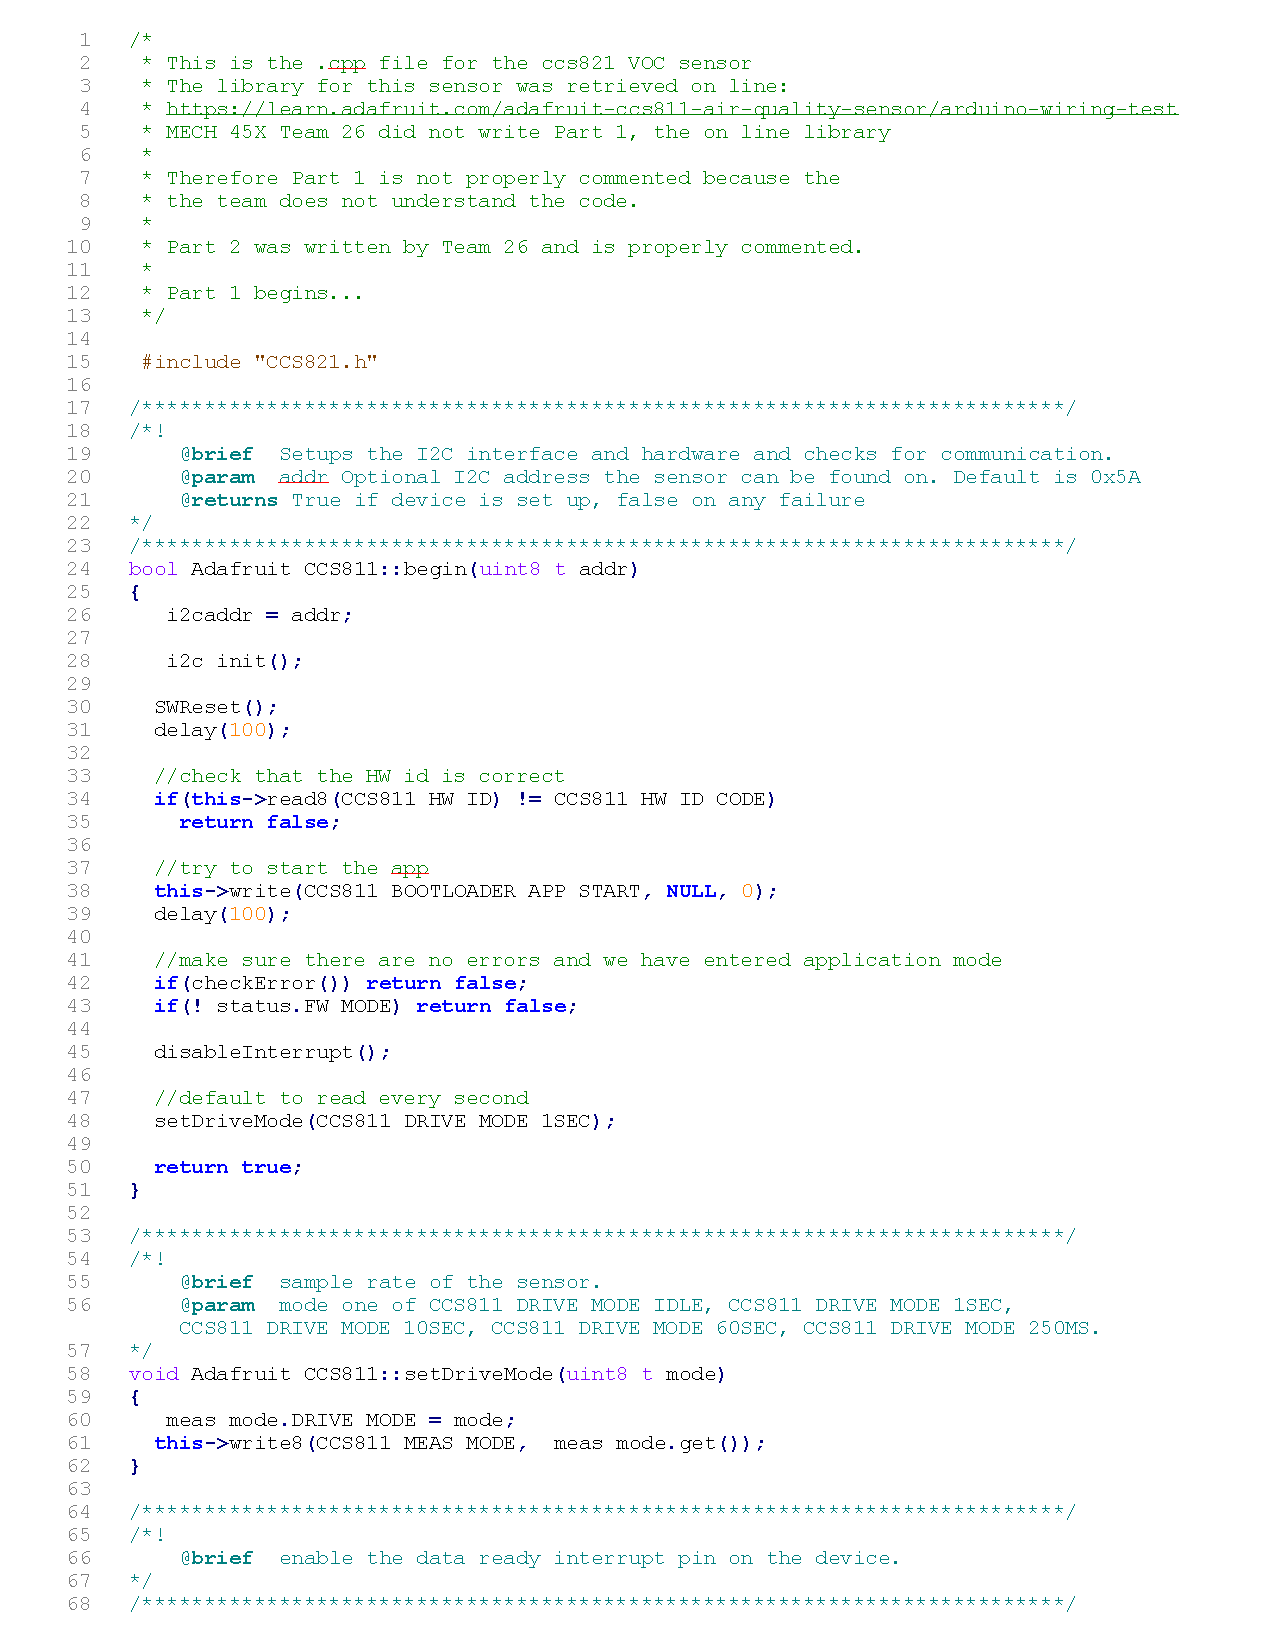
\includepdf[pages=-,pagecommand={},width=\textwidth]{ccs821_cpp.pdf}
% ****
% _SHT
% ****
The code for running the SHT35D Temperature and Relative Humidity sensor is:
\begin{verbatim}
'SHT35D.cpp' and 'SHT35D.h'
\end{verbatim}
This code reads from the SHT35D sensor several time and takes an average value of all of the readings. The SHT35D communicates using an I2C connection. This code was retrieved from:
\begin{verbatim}
https://github.com/closedcube/ClosedCube_SHT31D_Arduino
\end{verbatim}
The on line library was supplemented by additional methods added by Team 26. The .h file is presented first, followed by the .cpp file.
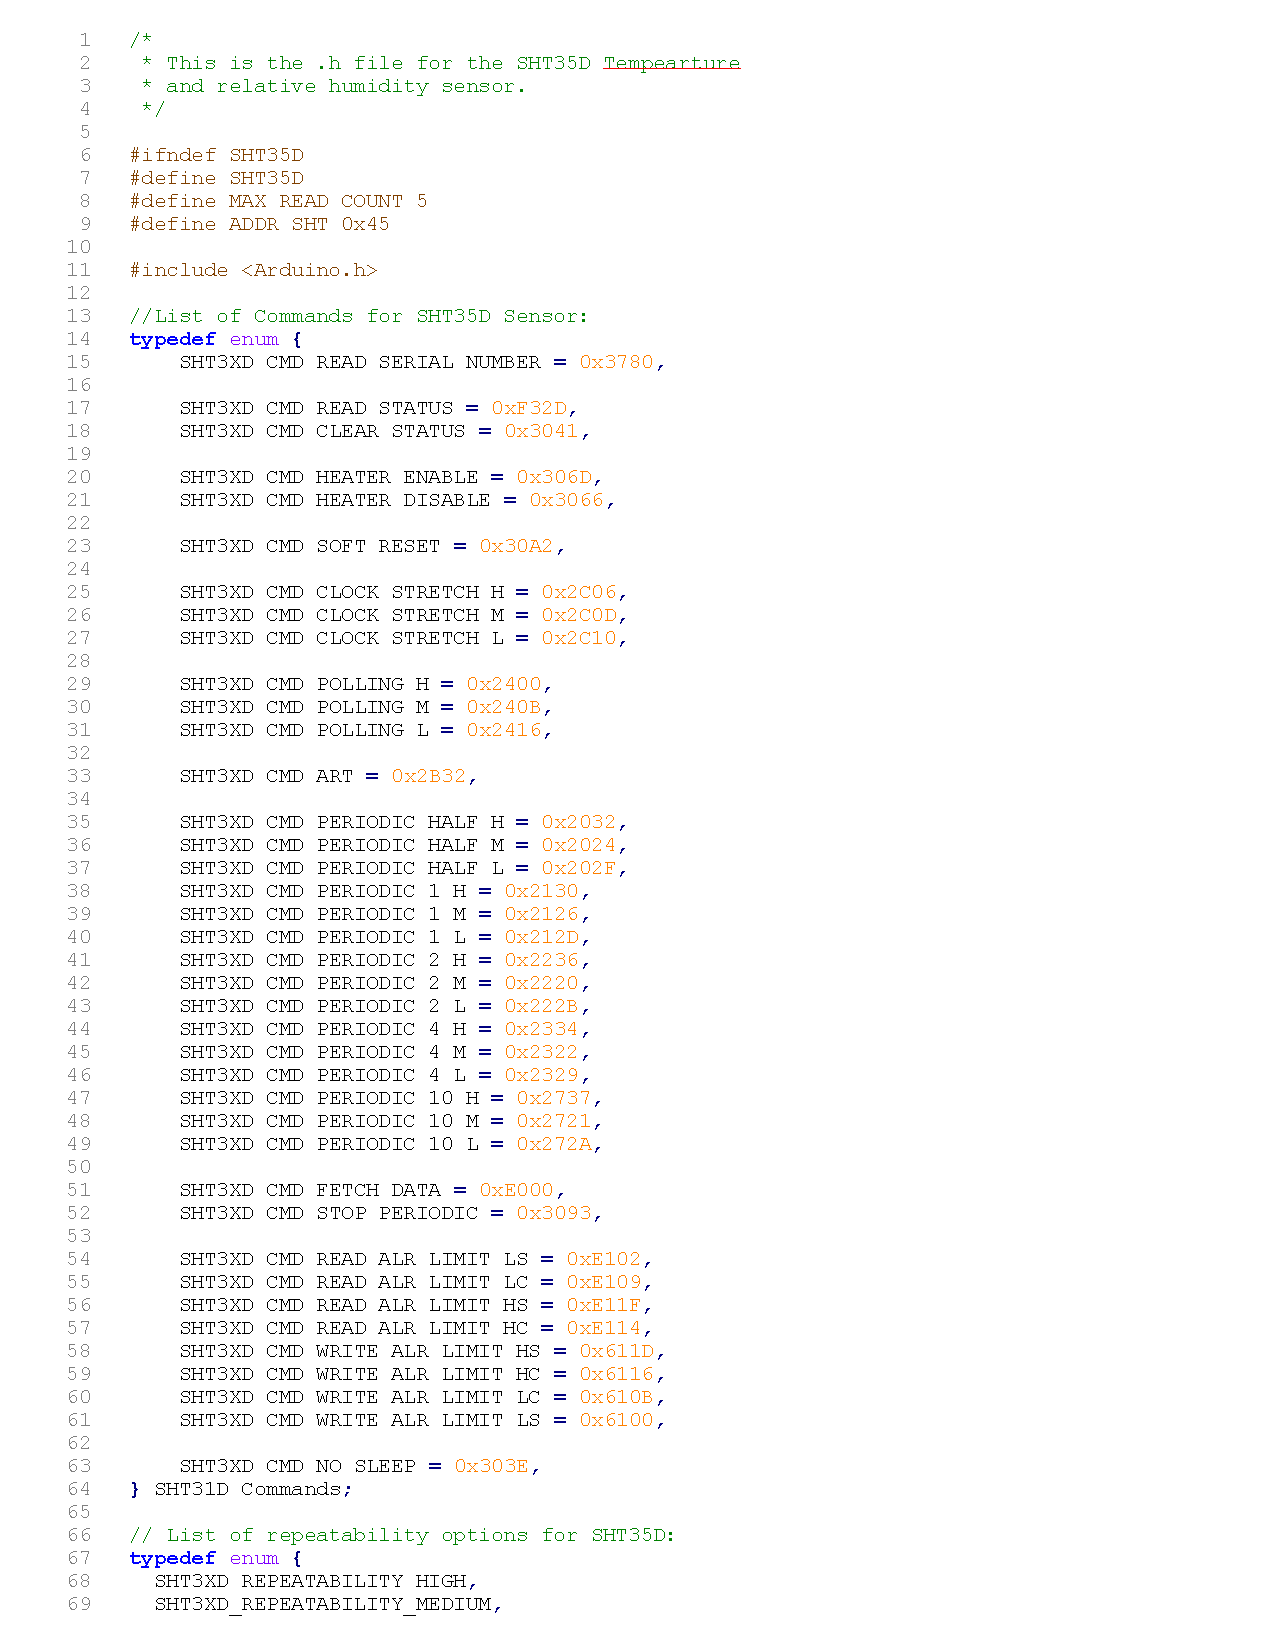
\includepdf[pages=-,pagecommand={},width=\textwidth]{SHT35D_h.pdf}
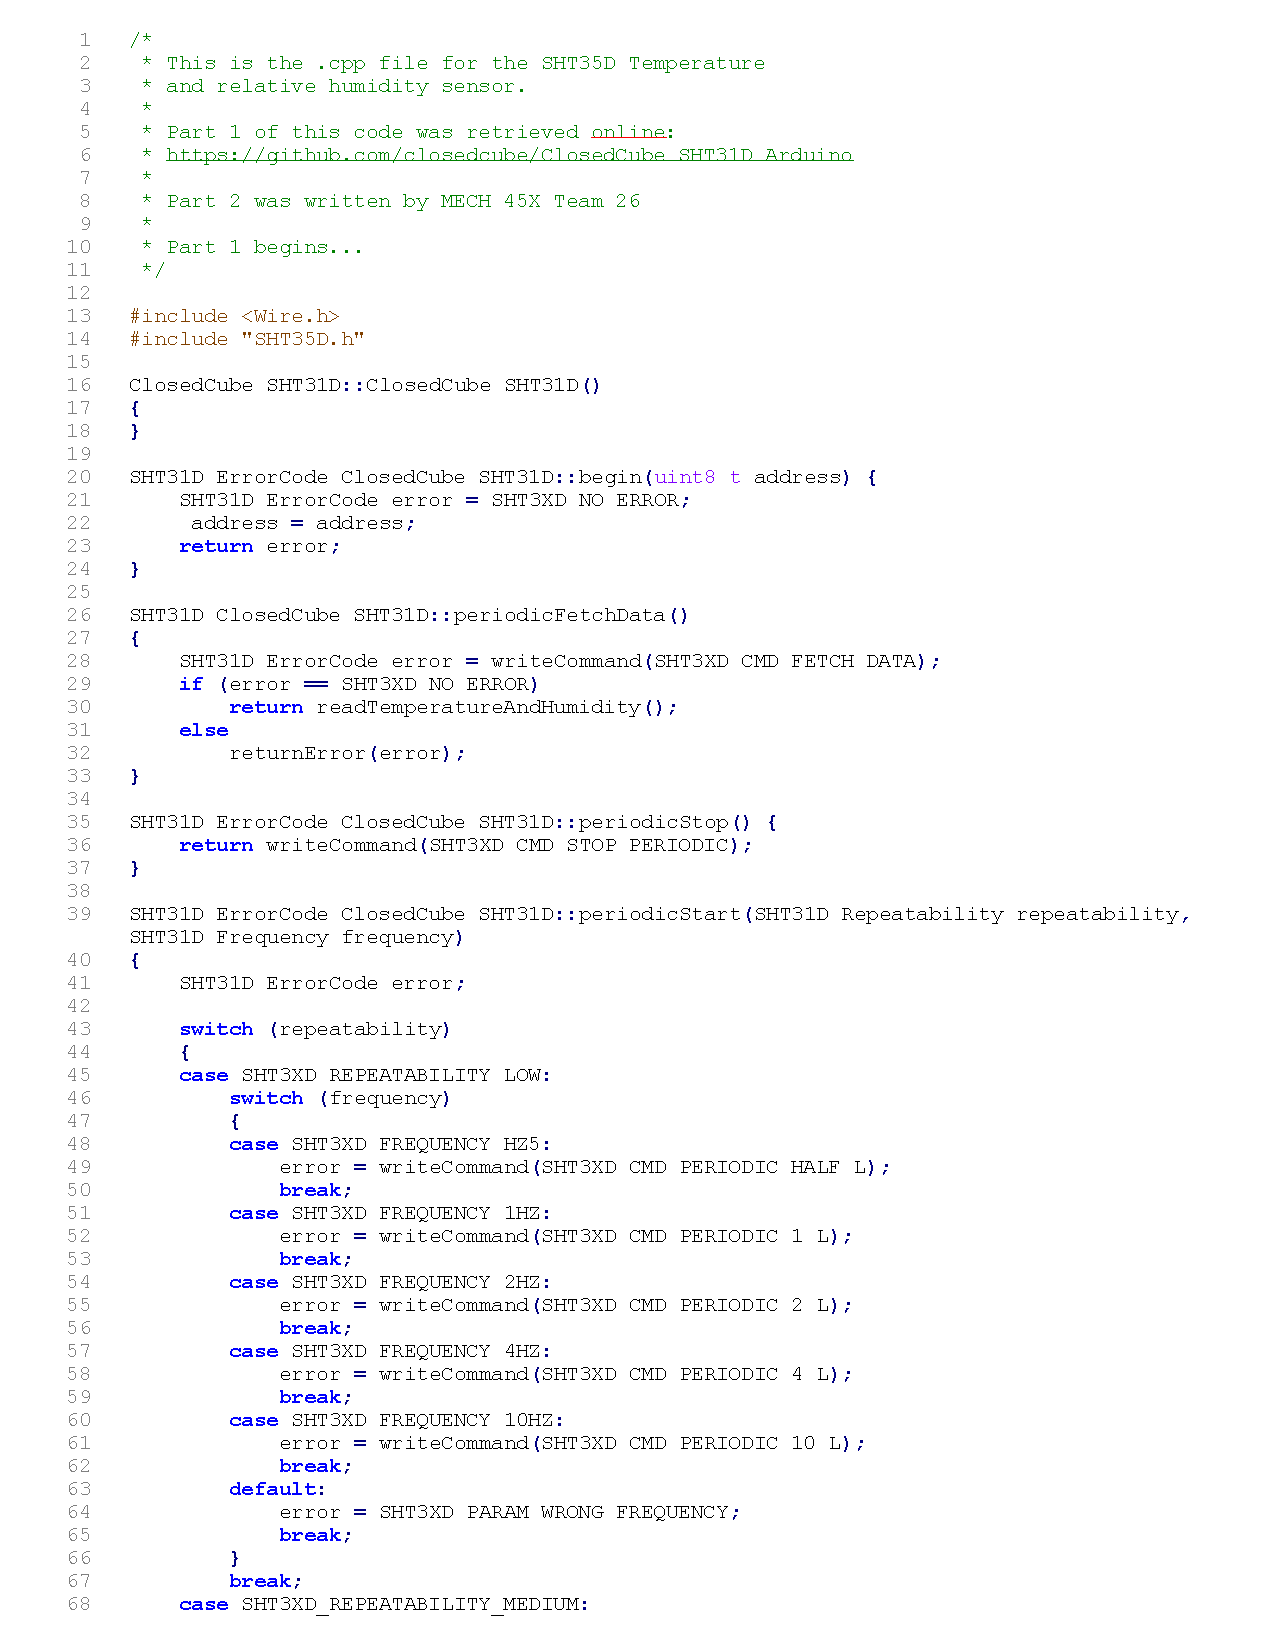
\includepdf[pages=-,pagecommand={},width=\textwidth]{SHT35D_cpp.pdf}
% ****
% _MRT
% ****
The code for running the Si7015 Globe Thermometer Temperature sensor:
\begin{verbatim}
'MRT.cpp' and 'MRT.h'
\end{verbatim}
This code reads from the Si7015 sensor several time and takes an average value of all of the readings. The Si7015 communicates using an I2C connection. This code was retrieved from:
\begin{verbatim}
https://github.com/closedcube/ClosedCube_Si7051_Arduino
\end{verbatim}
The on line library was supplemented by additional methods added by Team 26. The .h file is presented first, followed by the .cpp file.
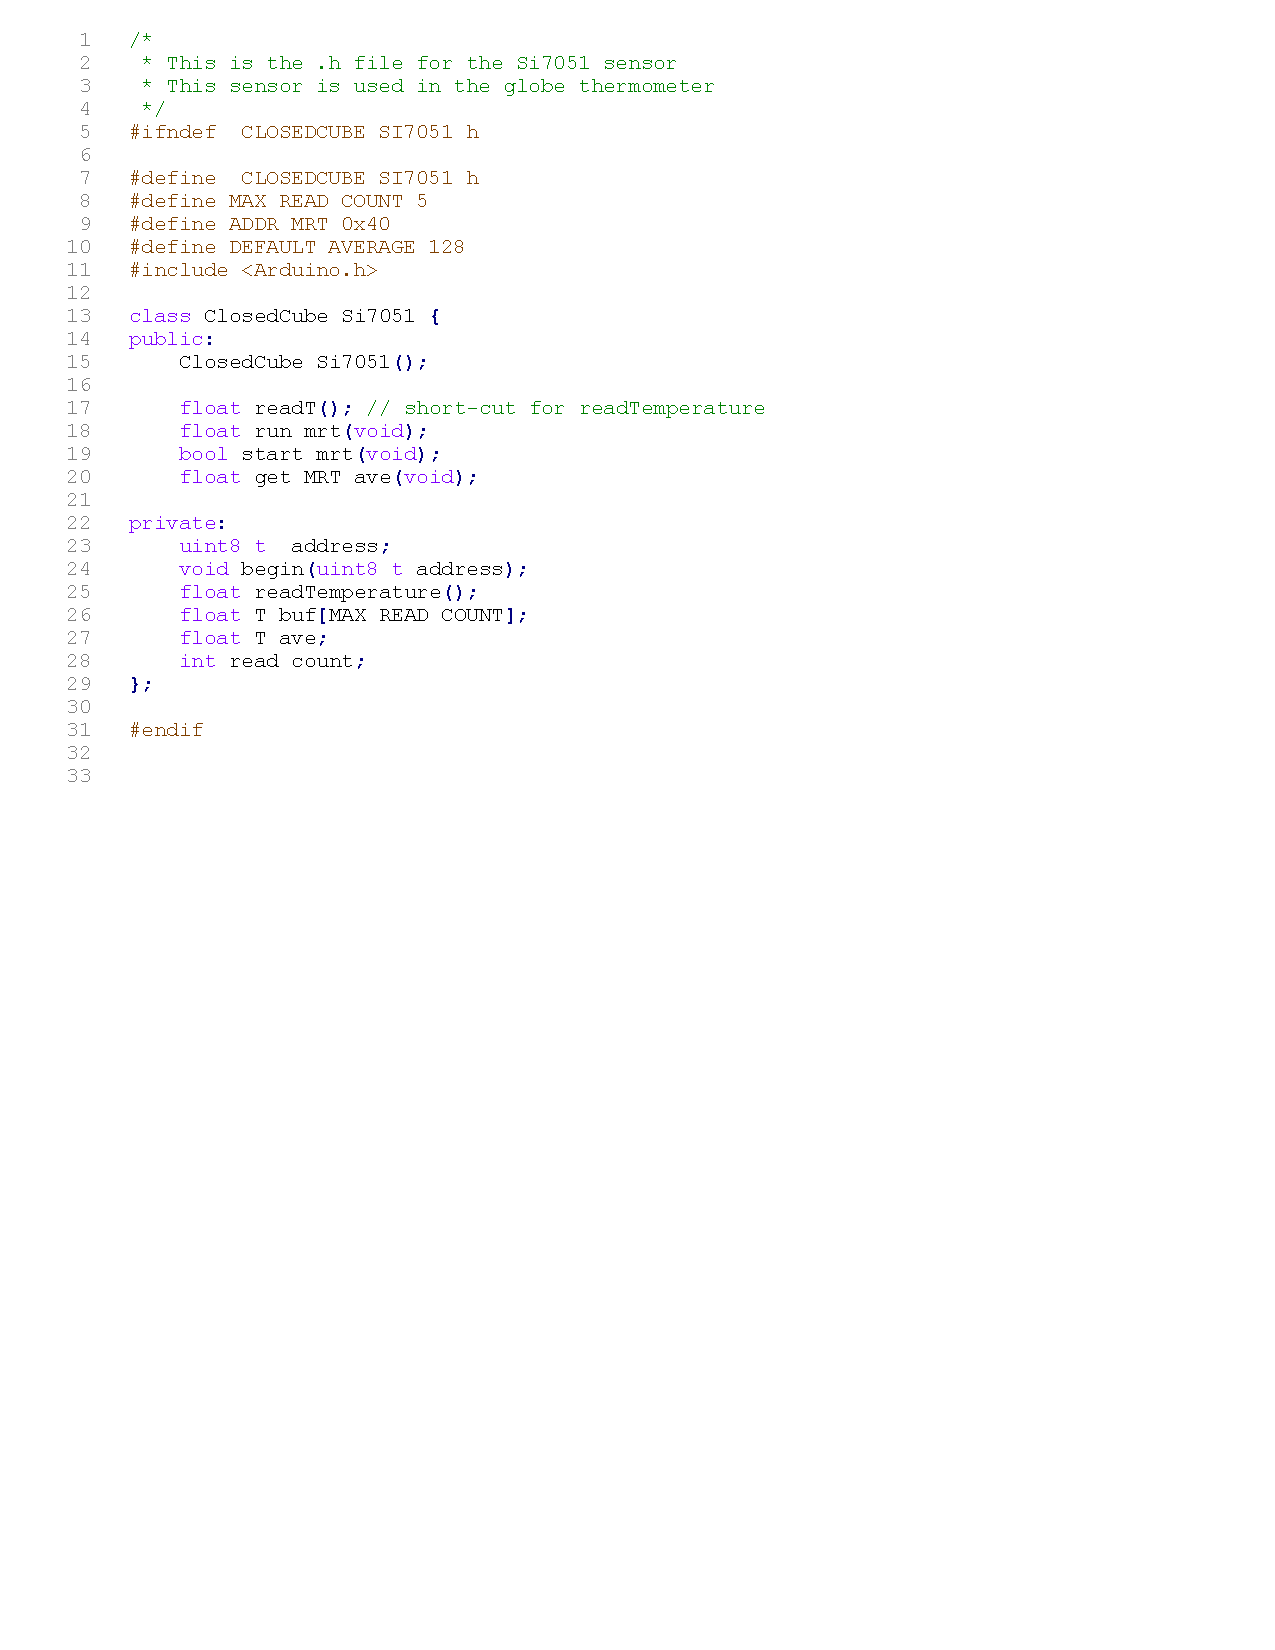
\includepdf[pages=-,pagecommand={},width=\textwidth]{MRT_h.pdf}
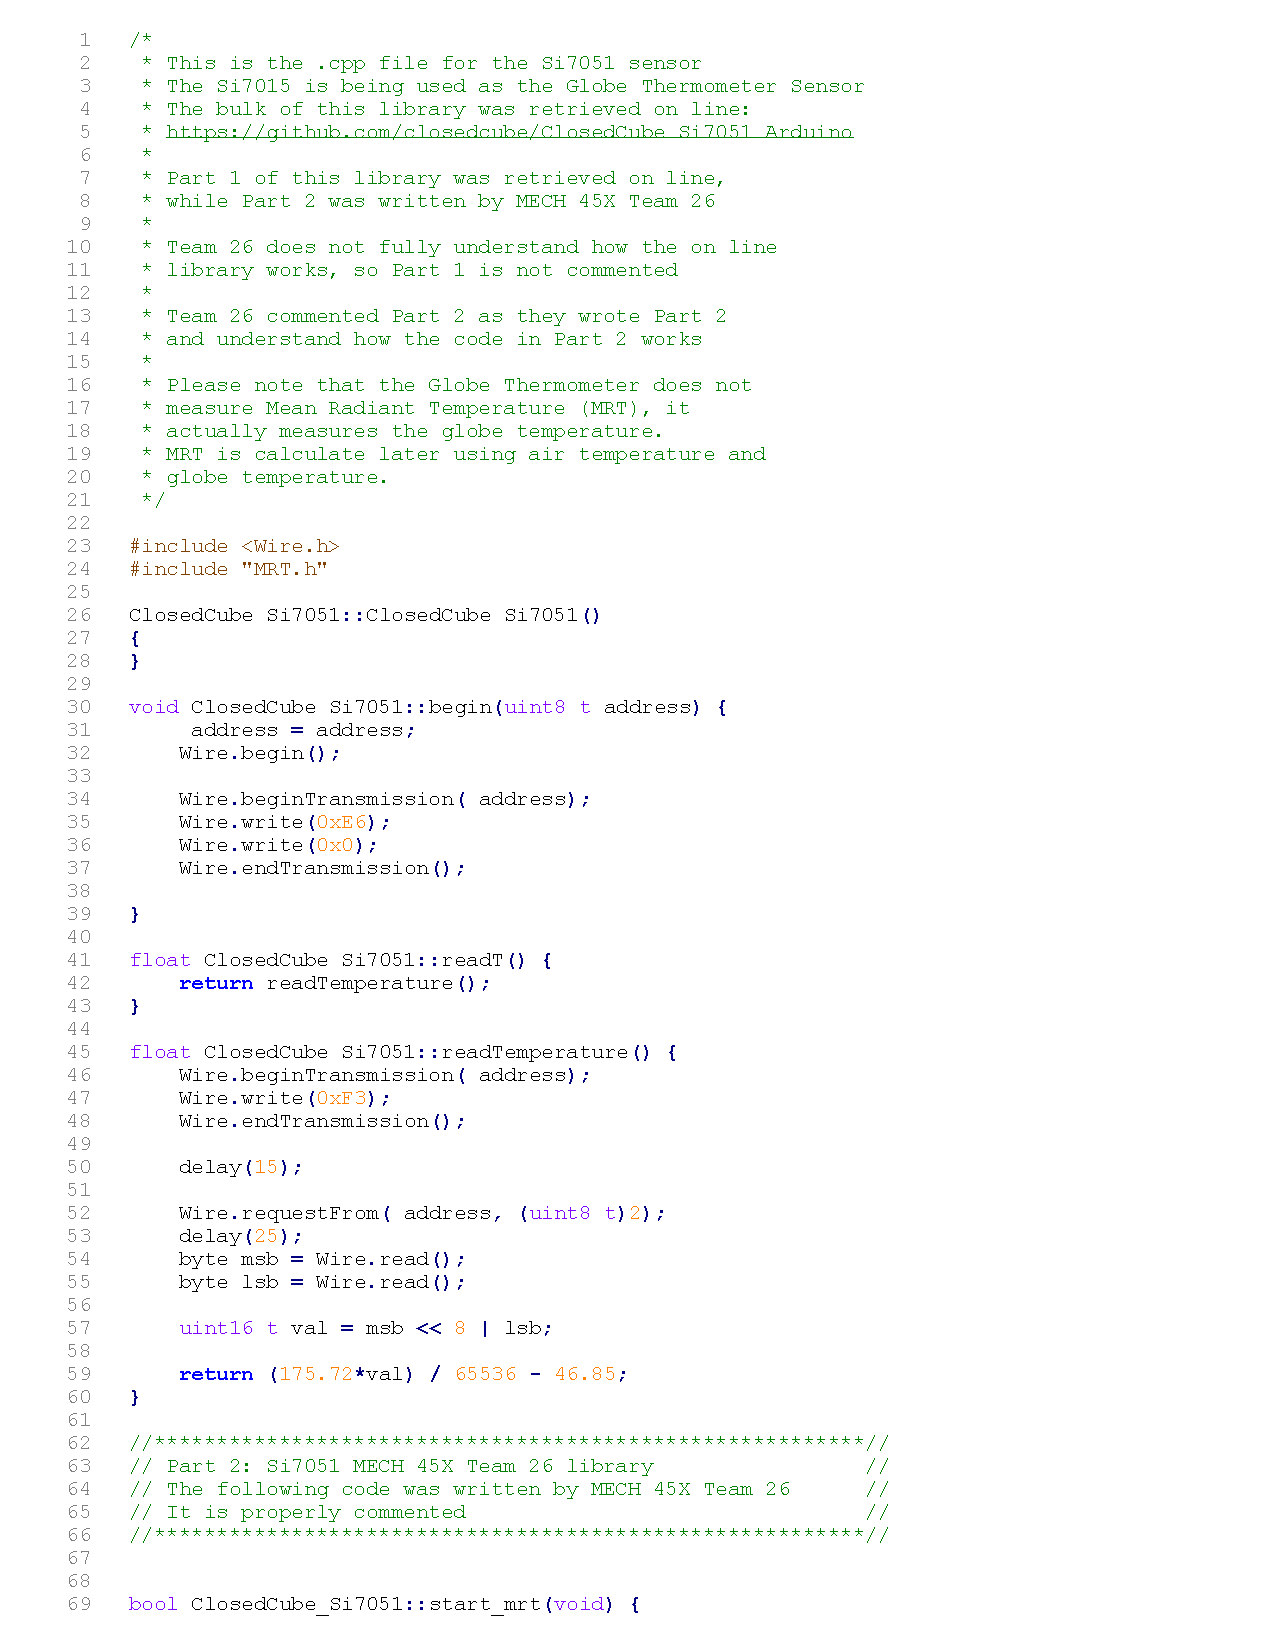
\includepdf[pages=-,pagecommand={},width=\textwidth]{MRT_cpp.pdf}
\end{document}